\documentclass{article}


\usepackage{PRIMEarxiv}

\usepackage[utf8]{inputenc} % allow utf-8 input
\usepackage[T1]{fontenc}    % use 8-bit T1 fonts
\usepackage{hyperref}       % hyperlinks
\usepackage{url}            % simple URL typesetting
\usepackage{booktabs}       % professional-quality tables
\usepackage{amsfonts}       % blackboard math symbols
\usepackage{amsthm}
\usepackage[linesnumbered,ruled,vlined]{algorithm2e}
\usepackage{amsmath}
\usepackage{hyperref}
\usepackage{nicefrac}       % compact symbols for 1/2, etc.
\usepackage{microtype}      % microtypography
\usepackage{lipsum}
\usepackage{fancyhdr}       % header
\usepackage{graphicx}
\usepackage{caption}
\usepackage{subcaption}
\usepackage{enumitem}
\usepackage{float}
% graphics
\graphicspath{{media/}}     % organize your images and other figures under media/ folder

 \hypersetup{
     colorlinks=true,
     linkcolor=blue,
     filecolor=blue,
     citecolor = black,
     urlcolor=cyan,
     }


\newtheorem{theorem}{Theorem}[section]
\newtheorem{corollary}{Corollary}[theorem]
\newtheorem{lemma}[theorem]{Lemma}
\newtheorem{definition}{Definition}[section]

\setlength{\parindent}{2em}

%Header
\pagestyle{fancy}
\thispagestyle{empty}
\rhead{ \textit{ }}

% Update your Headers here
\fancyhead[LO]{UGP, 21-22 Even Semester}
% \fancyhead[RE]{Firstauthor and Secondauthor} % Firstauthor et al. if more than 2 - must use \documentclass[twoside]{article}




%% Title
\title{Applications of Chatterjee's Correlation in MCMC
%%%% Cite as
%%%% Update your official citation here when published
%\thanks{\textit{\underline{Citation}}:
%\textbf{Authors. Title. Pages.... DOI:000000/11111.}}
}

\author{
  Vivek Kumar Singh \\
  Bachelor of Science \\
  Department of Mathematics and Statistics \\
  Indian Institute of Technology Kanpur \\
  % City\\
  \texttt{\{vksingh\}@iitk.ac.in} \\
  %% examples of more authors
   \And
  Dootika Vats \\
  Associate Professor \\
  Department of Mathematics and Statistics \\
  Indian Institute of Technology Kanpur \\
 % City\\
 \texttt{\{dootika\}@iitk.ac.in}
  %% \AND
  %% Coauthor \\
  %% Affiliation \\
  %% Address \\
  %% \texttt{email} \\
  %% \And
  %% Coauthor \\
  %% Affiliation \\
  %% Address \\
  %% \texttt{email} \\
  %% \And
  %% Coauthor \\
  %% Affiliation \\
  %% Address \\
  %% \texttt{email} \\
}


\begin{document}
\maketitle
\begin{abstract}
    Markov chain Monte Carlo (MCMC) algorithms are used to estimate features of interest of a distribution.
    The ACF used for assessing the quality of the produced chain and calculating the variance of Markov chain CLT is defined using Pearson correlation.
    In his recent paper, Chatterjee proposed a coefficient that solves some of Pearson correlation's problems.
    We present a new ACF defined using this coefficient and examine its behaviour on stationary Markov chains.
    We proved some results and sketched out a path for proving the consistency of the estimator of this ACF estimated using correlated draws.
\end{abstract}
\section{Introduction}

	Markov chain Monte Carlo (MCMC) methods are a class of algorithms used for sampling from complicated probability distributions.
	They are often required for parameter estimation in the statistical models encountered in real-world applications.

	If $X_1, X_2, \dots$ is a Markov chain,
	then the lag-k autocorrelation is defined as
	$$\gamma_k = \rho(X_1, X_{1+k}),$$
	where $\rho$ is Pearson's correlation coefficent (See Section 3).
	The autocorrelation function is used to measure the quality of the Markov chain produced.
	Pearson's correlation used above is great at detecting monotone relations in data,
	but doesn't perform well enough when applied to non-linear situations (say $\rho(X, \sin(X))$).

	Chatterjee proposed a new measure of dependence in \cite{chatterjee2020sourav}, which is
	(a) as simple as Pearson correlation,
	(b) is 0 if and only if the variables are independent and 1 if and only if one is a measurable function of the other, and
	(c) has a simple asymptotic theory under the hypothesis of independence, like Pearson correlation.
	See Section 4 for more on this.

	The advantages of this new measure motivated us to define a new autocorrelation function using Chatterjee's correlation coefficient instead of Pearson's.
	In order to use this in MCMC theory, two things were needed,\\
	1. Some properties that are followed by the classical ACF should also hold for our version for Markov chains.\\
	2. As we do not have the luxury of i.i.d. draws, for which the consistency of the estimator of Chatterjee's correlation holds (See \cite{chatterjee2020sourav}),
		we need to prove it for the case of MCMC samples we have.\\
	We proved three results for Chatterjee's correlation that are analogous to their Pearson counterpart (See Section 5).
	We also believe that the estimator for Chatterjee's correlation coefficient is consistent even when we are using correlated draws from a stationary Markov chain.
	Some ideas are presented (See Section 6) inspired by the proof of consistency in \cite{chatterjee2020sourav} of the i.i.d. estimator on how one should go about it.
	We were not able to complete it in this project and is left as future work.

\newpage
\section{Markov chain Monte Carlo}
	A Markov chain is a discrete time stochastic process $X_1, X_2, \dots$ taking values in an arbitrary general state space and having the Markov property,
	i.e. the conditional distribution of $X_{n+1}$ given the past $X_1, \dots X_n$, depends only on the present state $X_n$ (\cite{vats2017multivariate}).

	A Markov chain can be specified by two things, the intital distribution and the transition probabilities.
	The initial distribution is the marginal of $X_1$. By transition probabilities, we mean the conditional distribution of $X_{n+1}$ given $X_n$.
	We always assume stationary transition probabilities, i.e. the conditional $X_{n+1}|X_n$ is independent of $n$.\\
	A Markov chain is said to be stationary if the distribution of $X_n$ is independent of $n$,
	and ergodic if it converges to the invariant distribution regardless of the choice of the initial distribution.\\
	A stationary Markov chain is time-reversible w.r.t. the stationary distribution if $X_n$ and $X_{n+1}$ are exchangable (\cite{geyer2005charles}, \cite{mcmc2011handbook}).

\section{Pearson's Correlation Coefficient}
	Pearson correlation coefficient measures the linear correlation of two sets of data.
	Given a pair of random variables $(X, Y)$, Pearson correlation $\rho$ is defined as
	$$\rho = \frac{\Cov(X, Y)}{\sqrt{\Var[X]} \cdot \sqrt{\Var[Y]}}.$$

	Pearson's coefficent is very powerful in detecting monotone relations and
	has a well developed asymptotic theory. The autocorrelation function that we discussed about is also defined using this.

	\subsection{Problems with Pearson correlation}
		There are two most common problems with this coefficent.
		\begin{enumerate}
			\item First, we would like that the correlation would be close to its maximum value
			if and only if one variable looks like a noiseless function of the other variable.
			This is not the case as $\rho$ is close to $\pm 1$ iff one variable is a noiseless $\textit{linear}$ function.
			\item Second, we would like the correlation to be close to its minimum value if and only if both the variables are independent of each other.
			In the case of Pearson, it is zero when the variables are independent but the converse is not always true.
		\end{enumerate}

\section{Chatterjee's Correlation Coefficient}
	In order to solve these problems, Chatterjee came up with a new correlation coefficient (\cite{chatterjee2020sourav}, \cite{chatterjee2021mona}) which overcomes these drawbacks and also has a consistent estimator which is computationally efficient.\\
	Chatterjee's correlation $\xi$ is defined as
	$$\xi(X, Y) = \frac{\int Var(\mathbb{E}(1_{\{Y \geq t\}}|X)) d\mu(t)}{\int Var(1_{\{Y \geq t\}}) d\mu(t)},$$
	where $X, Y$ are any sets of random variables.

	\subsection{A consistent estimator of $\xi$}
		Let $(X, Y)$ be a pair of random variables, where Y is not a constant (for our purposes, both X and Y are continuous).
		Let $\{(X_i, Y_i)\}_{i = 1}^{n}$ be i.i.d. pairs following the same distribution as $(X, Y)$.
		\begin{enumerate}
			\item The case when $X_i's \text{ and } Y_i's$ have no ties: \\
			Rearrange the data as $(X_{(1)}, Y_{(1)}), \dots, (X_{(n)}, Y_{(n)})$ such that $X_{(1)} < \dots < X_{(n)}$. Let $r_i$ be the rank of $Y_{(i)}$, i.e. the number of $j$ such that $Y_{(j)} \leq Y_{(i)}$.  Then the correlation coefficient $\xi_n$ is defined to be
			$$\xi_n(X, Y) := 1-\frac{3\sum_{i=1}^{n-1} |r_{i+1} - r_i|}{n^2-1}.$$

			\item In the case of ties:\\
			If there are ties in $X_i's$, choose an increasing arrangement as follows and break ties uniformly at random. Let $r_i$ defined as above, and define $l_i$ to be the number of $j$ such that $Y_{(j)} \geq Y_{(i)}$. Define
			$$\xi_n(X, Y) := 1-\frac{n\sum_{i=1}^{n-1} |r_{i+1} - r_i|}{2\sum_{i=1}^{n-1}l_i(n-l_i)}.$$
			When there are no ties among the $Y_i's, l_1, \dots, l_n$ is just a permutation of $1, \dots, n$ and the denominator is just $n(n^2-1)/3$, which reduces to the definition in the no ties case.\\
		\end{enumerate}
		\begin{theorem}
			If $Y$ is not almost surely a constant, then as $n \rightarrow \infty$, $\xi_n(X, Y)$ converges almost surely to $\xi(X, Y)$, where $\mu$ is the pdf of $Y$.
		\end{theorem}
		Theorem 4.1 proves that $\xi_n$ is a consistent estimator of $\xi$. Proof is given in \cite{chatterjee2020sourav}.

	\subsection{Properties}
	Some properties of this new measure of dependence are as follows
	\begin{enumerate}
		\item $\xi(X, Y) \in [0, 1]$
		\item $\xi(X, Y) = 0$ if and only if $X$ and $Y$ are independent.
		\item $\xi(X, Y) = 1$ if and only if atleast one of $X$ and $Y$ is a measurable function of the other.
		\item $\xi_n$ is not symmetric in $X, Y$. This is intentional and useful as we might want to study if $Y$ is a measurable function of $X$, or $X$ is a measurable function of $Y$. To get a symmetric coefficient, it suffices to consider $\max(\xi_n(X, Y), \xi_n(Y, X))$.
		\item $\xi_n$ is based on ranks, and for the same reason, it can be computed in $O(n\log n)$.
	\end{enumerate}

\section{Chatterjee's Autocorrelation Function}
	The aim of this project is to create a new autocorrelation function (ACF) using Chatterjee's correlation coefficient, and study it's behaviour when applied to Markov chains.\\
	Let $X_1, X_2, \dots$ be a stationary, time homogeneous Markov chain with stationary distribution $\pi$.
	We define the new lag-k ACF as follows
	$$\gamma_{k, n}' := \xi(X_n, X_{n+k}).$$

	\begin{theorem}
		Here we present a proof of a well known result about Pearson Correlation Coefficient.
		$$\Cov(X_n, X_{n+k}) \text{ is independent of } n.$$
		\begin{proof}
			We know that
			$$\Cov(X_n, X_{n+k}) = \mathbb{E}[X_n X_{n+k}] - \mathbb{E}[X_n]\mathbb{E}[X_{n+k}].$$
			Also, as $X_n$ is a stationary markov chain, $\mathbb{E}[X_n] = \mu$, where $\mu$ is the mean of the distribution $\pi$.\\
			And,
			$$\mathbb{E}[X_n X_{n+k}] = \int\int xyf_{(X_n, X_{n+k})}(x, y)dxdy$$
			where $f_{(X_n, X_{n+k})}$ is the joint density of $X_n$ and $X_{n+k}$. Now as the markov chain is stationary, this density is dependent only on $k$, i.e. $$f_{(X_k, X_{k+n})} = f_{(X_1, X_{1+n})}.$$
			As both the terms of $\Cov(X_n, X_{n+k})$ are independent of $n$, $\Cov(X_n, X_{n+k})$ is independent of $n$.\\
		\end{proof}
	\end{theorem}
	This theorem is important as it allows us to estimate the ACF without drawing multiple Markov chains.
	This suggests that the same property should also hold for $\gamma_{k, n}'$, proved in the next theorem.
	\newpage
	\begin{theorem}
		$\xi(X_n, X_{n+k})$ is independent of $n$, where $n$ and $k$ are in $\mathbb{N}$.
		\begin{proof}
			\begin{equation}
				\xi_{(X_n, X_{n+k})} = \frac{\int \Var[\mathbb{E}[1_{\{X_{n+k} \geq t\}}|X_n=x]] d\pi(t)}{\int \Var[1_{\{X_{n+k} \geq t\}}] d\pi(t)}.
			\end{equation}
			We'll prove that both the numerator and the denominator are independent of $k$. \\
			We can write
			\begin{equation*}
				\mathbb{E}[1_{\{X_{n+k} \geq t\}}|X_n=x] = \Pr(X_{n+k} \geq t|X_n=x) \\
			\end{equation*}
			and by time-homogeneity of our Markov chain
			\begin{equation*}
				\Pr(X_{n+k} \geq t|X_n=x) = \int_t^{\infty} P^k(x, dy)
			\end{equation*}
			which is independent of $n$. And hence,
			\begin{equation}
				\int \Var\left[ \int_t^{\infty} P^k(x, dy)\right] d\pi(u)
			\end{equation}
			is also independent of $n$.\\\\
			Now for the denominator, we know by stationarity of our Markov chain that $X_n \sim \pi$, so for any function $f, f(X_n) \sim \pi'$ for some distribution $\pi'$, and therefore the variance will be same for all $n$.\\
			Let $f_t: \mathbb{R} \rightarrow \mathbb{R}$ such that $f_t(X) = 1_{\{X \geq t\}}$.\\
			We can write the denominator as
			$$\int \Var[f_t(X _{n+k})] d\pi(t)$$
			where,
			$$\Var[f_t(X_{n+k})] = \Var[f_t(X_{1})].$$
			Therefore,
			$$\int \Var[f_t(X_{n+k})] d\pi(t)$$
			is independent of both $n$ and $k$.\\\\
			As both the numerator and denominator are independent of $n$, we can conclude that $\xi(X_n, X_{n+k})$ is independent of $n$.
		\end{proof}
	\end{theorem}
	Because of Theorem 5.2, we can safely denote this new ACF by $\gamma_k'$.

	Now, if the Central Limit Theorem holds for a Markov chain, the variance is as follows
	$$\sigma_{\text{clt}}^2 = \sum_{k=-\infty}^{\infty} \gamma_k.$$

	As $\gamma_k$ is symmetric, we get that
	$$\sigma_{\text{clt}}^2 = \gamma_0 + 2\sum_{k=1}^{\infty} \gamma_k.$$
	Now $\xi$ is not symmetric in general, but for our purposes, it'd be great to have symmmetricity so that we can do a similar step as above.
	We've proved the symmmetricity of $\xi$ in the case of time reversible Markov chains.

	\begin{theorem}
		$\xi(X_n, X_{n+k}) = \xi(X_{n+k}, X_n)$ for time reversal Markov chains for any $n, k \in \mathbb{N}$.
		\begin{proof}
			By Theorem 5.2, we know that the denominator of $\xi(X_n, X_{n+k})$ is independent of both $n$ and $k$. So we only have to prove that the numerator is symmetric. \\
			We have to show that
			\begin{equation*}
				\int \Var [\Pr (X_{n+k} \geq t | X_n)] d\pi(t) = \int \Var [\Pr (X_n \geq t | X_{n+k})] d\pi(t).
			\end{equation*}
			\begin{lemma}
				For a time reversible Markov chain, $X_n$ and $X_{n+k}$ are exchangable, i.e.
				\begin{equation*}
					f_{(X_{n}, X_{n+k})}(x, y) = f_{(X_{n+k}, X_{n})}(x, y) \text{  } \forall (x, y) \in \mathbb{R}^2.
				\end{equation*}
				\begin{proof}
					It is enough to show that for any two $A, B \in \mathcal{B}(\mathbb{R})$
					\begin{align*}
						\Pr(X_n \in A, X_{n+k} \in B) = \Pr(X_{n+k} \in A, X_{n} \in B)
					\end{align*}
					which is same as
						$$\int_A \pi(dx) P^k(x, B) = \int_B \pi(dy) P^k(y, A)$$
						$$\Longleftrightarrow\int_A \int_B \pi(dx) P^k(x, dy) = \int_B \int_A \pi(dy) P^k(y, dx).$$
					To prove the above statement, it is enough to show that for any $x \in A$ and $y \in B$,
					$$\pi(dx) P^k(x, dy) = \pi(dy) P^k(y, dx).$$
					We proceed by strong induction on $k$.
					For $k = 1$, it is true by definition of reversibility of Markov chains.\\
					Assume that it is true for all $1 \leq m < k$.
					We want to prove it for $k$.\\
					By Chapman-Kolmogorov equation (\cite{mcmc2011handbook}), we have
					\begin{align*}
						\pi(dx) P^k(x, dy) &= \pi(dx) \int_{\mathcal{X}} P^m(x, dz)\cdot P^{k-m}(z, dy)\\
						&= \int_{\mathcal{X}} \pi(dx) P^m(x, dz) P^{k-m}(z, dy)
					\end{align*}
					by the inductive hypothesis, we get
					\begin{align*}
						&= \int_{\mathcal{X}} \pi(dz) P^m(z, dx) P^{k-m}(z, dy) \\
						&= \int_{\mathcal{X}} P^m(z, dx) \pi(dz) P^{k-m}(z, dy) \\
						&= \int_{\mathcal{X}} P^m(z, dx) \pi(dy) P^{k-m}(y, dz) \\
						&= \pi(dy) \int_{\mathcal{X}}  P^{k-m}(y, dz) P^m(z, dx)
					\end{align*}
					again by Chapman-Kolmogorov equation, we get that
					\begin{align*}
						&= \pi(dy) \cdot P^k(y, dx).
					\end{align*}
				\end{proof}
			\end{lemma}
			By Lemma 5.4, it is clear that
			\begin{equation*}
				\Pr (X_{n+k} \geq t | X_n) = \Pr (X_n \geq t | X_{n+k}) \text{  } \forall t \in \mathbb{R}
			\end{equation*}
			which implies the result above.
		\end{proof}
	\end{theorem}

	For an Ergodic Markov chain, we can intuitively argue that the correlation should approach $0$ as the time difference increases.
	In the next theorem, we've proved that this holds true for $\xi$.
	\begin{theorem}
		$\lim_{n \rightarrow \infty} \xi(X_1, X_{n}) = 0$ for an Ergodic Markov chain.
		\begin{proof}
			We have
			\begin{equation*}
				\xi(X_1, X_{n}) = \frac{\int \Var[\mathbb{E}[1_{\{X_{n} \geq t\}}|X_1=x]] d\pi(t)}{\int \Var[1_{\{X_{n} \geq t\}}] d\pi(t)}.
			\end{equation*}
			The denominator is independent of $n$ as proven in Theorem 5.2, so we only need to show that the numerator goes to 0 as $n \rightarrow \infty$.\\
			\begin{lemma}
				$$\lim_{n \rightarrow \infty} \int \Var[\mathbb{E}[1_{\{X_{n} \geq t\}}|X_1=x]] d\pi(t) = \int \lim_{n \rightarrow \infty}\Var[\mathbb{E}[1_{\{X_{n} \geq t\}}|X_1=x]] d\pi(t).$$
				\begin{proof}
					Define $f_n(t) := \Var[\Pr(X_{n} \geq t | X_{1} = x)] \cdot \pi(t)$. \\
					It is easy to see that $f_n$ is measurable, $\int_{-\infty}^{\infty} f_n < \infty$ and $f_n$ is continuous.\\
					Now, as $f_n$ is a product of two bounded functions, it is also bounded.
					Set
					$$ C:= \sup_{n \in \mathbb{N}} \left(\sup_{t \in \mathbb{R}} \left(\Var[\Pr(X_{n} \geq t | X_{1} = x)]\right)\right)$$
					then
					$$\int_{-\infty}^{\infty} f_n(t)dt \leq \int_{-\infty}^{\infty} C\cdot\pi(t)dt = C < \infty.$$
					As $f_n$ is dominated by $g$ (where $g(t) := C\cdot\pi(t) \forall t \in \mathbb{R})$, \\
					by Lebesgue's Dominated Convergence Theorem (\cite{kl2001chung}),
					$$\lim_{n \rightarrow \infty} \int f_n(t) dt = \int \left(\lim_{n \rightarrow \infty} f_n(t)\right) dt.$$
				\end{proof}
			\end{lemma}
			\begin{lemma}
				$$\lim_{n \rightarrow \infty} \Var[\mathbb{E}[1_{\{X_{n} \geq t\}}|X_1=x]] = \Var\left[\lim_{n \rightarrow \infty} \mathbb{E}[1_{\{X_{n} \geq t\}}|X_1=x]\right].$$
				\begin{proof}
					We can write
					\begin{align*}
						\Var[\mathbb{E}[1_{\{X_{n} \geq t\}}|X_1=x]] &= \mathbb{E}[\mathbb{E}[1_{\{X_{n} \geq t\}}|X_1=x]^2] - \mathbb{E}[\mathbb{E}[1_{\{X_{n} \geq t\}}|X_1=x]]^2 \\
						&= \mathbb{E}[\Pr(X_{n} \geq t | X_{1} = x)^2] - \mathbb{E}[\Pr(X_{n} \geq t | X_{1} = x)]^2.
					\end{align*}
					Assuming that both $\lim_n \mathbb{E}[\Pr(X_{n} \geq t | X_{1} = x)^2]$ and  $\lim_n \mathbb{E}[\Pr(X_{n} \geq t | X_{1} = x)]^2$ exist,
					\begin{align*}
						\lim_{n \rightarrow \infty} \Var[\mathbb{E}[1_{\{X_{n} \geq t\}}|X_1=x]] &= \lim_{n \rightarrow \infty} \mathbb{E}[\Pr(X_{n} \geq t | X_{1} = x)^2]\\
						&- \lim_{n \rightarrow \infty} \mathbb{E}[\Pr(X_{n} \geq t | X_{1} = x)]^2\\
						&= \lim_{n \rightarrow \infty} \mathbb{E}[\Pr(X_{n} \geq t | X_{1} = x)^2]\\
						&- \left(\lim_{n \rightarrow \infty} \mathbb{E}[\Pr(X_{n} \geq t | X_{1} = x)]\right)^2.\\
					\end{align*}
					For any $n \in \mathbb{N}$, we can write
					$$\mathbb{E}[\Pr(X_{n} \geq t | X_{1} = x)^n] = \int_{-\infty}^{\infty} \Pr(X_{n} \geq t | X_{1} = x)^n \cdot \pi(t)dt.$$
					\begin{lemma}
						$$\lim_{n \rightarrow \infty} \int \Pr(X_{n} \geq t | X_{1} = x)^n \cdot \pi(t) dt = \int \lim_{n \rightarrow \infty}\Pr(X_{n} \geq t | X_{1} = x)^n \cdot \pi(t)dt.$$
						\begin{proof}
							Define $f_n(t) := \Pr(X_{n} \geq t | X_{1} = x)^n \cdot \pi(t)$. \\
							It is easy to see that $f_n$ is measurable, $\int_{-\infty}^{\infty} f_n < \infty$ and $f_n$ is continuous.\\
							Now, as $f_n$ is a product of two bounded functions, it is also bounded. \\
							Now,
							$$\int_{-\infty}^{\infty} f_n(t)dt \leq \int_{-\infty}^{\infty} \pi(t)dt = 1 < \infty.$$
							As $f_n$ is dominated by $\pi$, \\
							by Lebesgue's Dominated Convergence Theorem,
							$$\lim_{n \rightarrow \infty} \int f_n(t) dt = \int \left(\lim_{n \rightarrow \infty} f_n(t)\right) dt.$$
						\end{proof}
					\end{lemma}
					Using Lemma 5.8 for $n = 1$ and $2$, we can take limit in both the terms inside, i.e.
					\begin{align*}
						\lim_{n \rightarrow \infty} \Var[\mathbb{E}[1_{\{X_{n} \geq t\}}|X_1=x]] &= \lim_{n \rightarrow \infty} \mathbb{E}[\Pr(X_{n} \geq t | X_{1} = x)^2]\\
						&- \left(\lim_{n \rightarrow \infty} \mathbb{E}[\Pr(X_{n} \geq t | X_{1} = x)]\right)^2\\
						&= \mathbb{E}\left[\lim_{n \rightarrow \infty} \Pr(X_{n} \geq t | X_{1} = x)^2\right]\\
						&- \left(\mathbb{E}\left[\lim_{n \rightarrow \infty}\Pr(X_{n} \geq t | X_{1} = x)\right]\right)^2\\
						&= \Var\left[\lim_{n \rightarrow \infty} \mathbb{E}[1_{\{X_{n} \geq t\}}|X_1=x]\right].
					\end{align*}
				\end{proof}
			\end{lemma}
			Now we know that
			\begin{equation*}
				\mathbb{E}[1_{\{X_{n} \geq t\}}|X_1=x] = \int_t^{\infty} P^{n-1}(x, dy)
			\end{equation*}
			For an Ergodic Markov chain, under the Total Variation Norm, we know that for every initial distribution $\lambda$
			\begin{equation*}
				\lim_{k\rightarrow\infty}||\lambda P^k - F|| = 0.
			\end{equation*}
			Consequently, for all $x \in \mathbb{R}$,
			\begin{equation*}
				\lim_{k\rightarrow\infty}||P^k(x, \cdot) - F(\cdot)|| = 0.
			\end{equation*}
			So, define $$G_{k, x}(t) := \int_{-\infty}^{t} P^{k}(x, dy)$$
			i.e. the cdf of $P^k(x, \cdot)$. By ergodicity, we get that
			$$G_{k, x}(t) \xrightarrow{d} F(t).$$
			This implies
			\begin{align*}
				\lim_{n \rightarrow \infty} \int \Var\left[\mathbb{E}[1_{\{X_{n} \geq t\}}|X_1=x]\right] d\pi(t) &= \lim_{n \rightarrow \infty} \int \Var\left[\int_t^{\infty} P^{n-1}(x, dy)\right] d\pi(t)\\
				&= \lim_{n \rightarrow \infty} \int \Var\left[1-G_{n-1, x}\right] d\pi(t)\\
				&= \int \Var\left[\lim_{n \rightarrow \infty}(1-G_{n-1, x})\right] d\pi(t)\\
				&= \int \Var\left[1-F(t)\right] d\pi(t)\\
				&= \int 0 \cdot d\pi(t)\\
				&= 0.
			\end{align*}
		\end{proof}
	\end{theorem}

\section{Proof sketch of Theorem 4.1 for correlated samples}
	Chatterjee presented the complete proof of Theorem 4.1 in \cite{chatterjee2020sourav}, where the samples drawn from $(X, Y)$ are i.i.d.
	In our case of MCMC, for the estimation of Chatterjee's correlation, we have correlated but identically distributed draws due to stationarity.
	To use this new autocorrelation function, we need to estimate it first, and for that, we need the estimator to be consistent in our case.
	We aim to prove that the estimator is consistent even in the stationary Markov chain case.
	We believe that the convergence does happen but could not prove it completely in this project, and it is left as future work.

	\begin{theorem}
		Let $X_1, X_2, \dots$ be a stationary time-homogeneous Markov chain with stationary distribution $\mu$.
		Then $\xi_n(X, Y)$ estimated using the draws from the Markov chain converge to $\xi(X, Y)$ as $n \rightarrow \infty$, where X, Y are any two time points in the chain.
	\end{theorem}
	All the Lemmas and Corollaries are taken directly from the proof in the i.i.d. case given in \cite{chatterjee2020sourav}.
	\begin{proof}
		Lemma 9.1 and Corollary 9.2 of \cite{chatterjee2020sourav} follow directly without any changes.

        We could not prove Lemma 9.3, but we believe that it can be proven and is left for the future.

        We proved Lemma 9.4 in the case of stationary Markov chain. The only place where the i.i.d. property of $\{X_n\}$ was used is to show that
		$$\frac{1}{n}\sum_{j = 1}^{n}\mathbb{E}(f(X_j)) = \mathbb{E}(f(X_1)).$$
		This statement is also true in the case of stationary Markov chains, and hence we are done.

        Lemma 9.5 is a special case of Lusin's Theorem (See \cite{chatterjee2020sourav}).

        Lemma 9.6 requires Lemma 9.3, 9.4 and 9.5. If we can prove Lemma 9.3, we are done.

        Lemma 9.7 is a standard probability result.

        Proof of Lemma 9.8 requires i.i.d. samples and Lemma 9.7. We were not able to prove Lemma 9.8 for our case.

        We get Corollary 9.9 by adding the results of Lemma 9.6 and Lemma 9.8.

        Lemma 9.10 requires Corollary 9.9 and the Glivenko-Cantelli theorem. As we have an ergodic Markov chain version of the Glivenko-Cantelli version,
        we are done after proving Corollary 9.9.

        Proof of Lemma 9.11 also does not require any modifications from the one given in \cite{chatterjee2020sourav}.

        Corollary 9.12 follows directly from Lemma 9.10 and Lemma 9.11.

        The proof of the main theorem requires the Glivenko-Cantelli theorem, Corollary 9.2 and Corollary 9.12.
        The future work is to prove Lemma 9.3 and Lemma 9.8, and we will be done.

	\end{proof}

\section{Simulations}
	Assuming Theorem 6.1, we've presented below two sets of ACF plots of two different Markov chains.
	On the left column, we have Pearson's ACF plot, and on the right we have Chatterjee's ACF plot.

	First, we have the AR(1) process with $\rho = 0.8$.
	\begin{figure}[H]
		\centering
		\begin{subfigure}[b]{0.4\linewidth}
			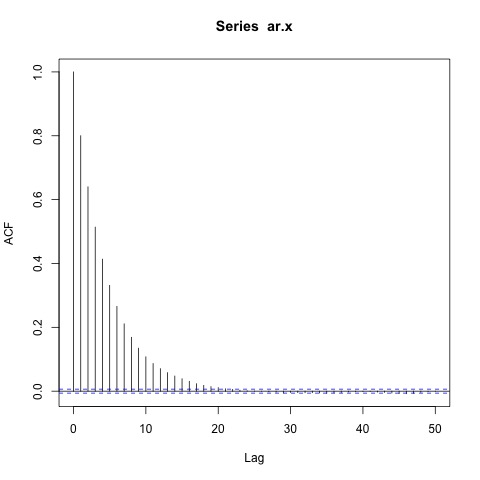
\includegraphics[width=\linewidth]{acf_ar.jpg}
			\caption{Classical ACF}
		\end{subfigure}
		\begin{subfigure}[b]{0.4\linewidth}
			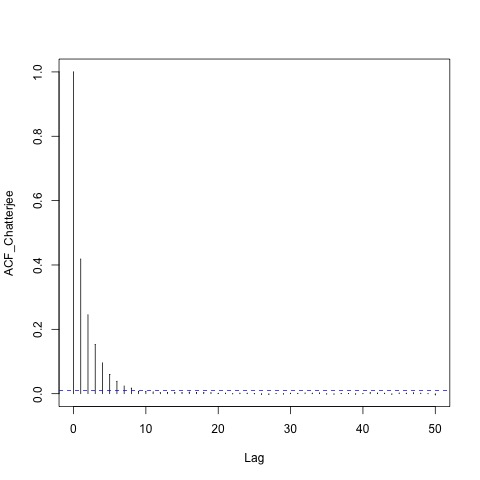
\includegraphics[width=\linewidth]{acf_ar_chatterjee.jpg}
			\caption{Chatterjee's ACF}
		\end{subfigure}
		\caption{AR(1) Process with $\rho = 0.8$}
		\label{fig:ar_acf}
	\end{figure}

	Next, we have the Metropolis-Hastings algorithm with initial distribution as Exp(0.01) and target distribution $\mathcal{N}(0, 1)$
	\begin{figure}[H]
		\centering
		\begin{subfigure}[b]{0.4\linewidth}
			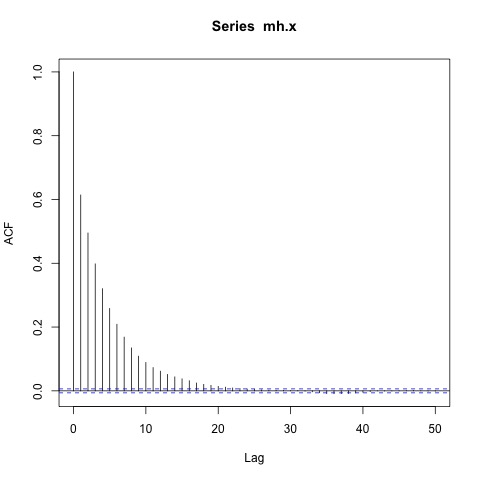
\includegraphics[width=\linewidth]{acf_mh.jpg}
			\caption{Classical ACF}
		\end{subfigure}
		\begin{subfigure}[b]{0.4\linewidth}
			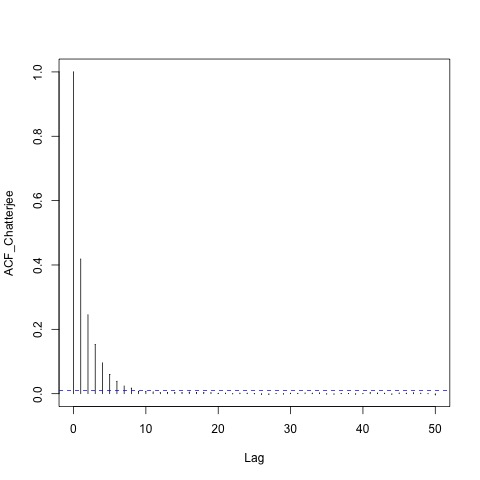
\includegraphics[width=\linewidth]{acf_mh_chatterjee.jpg}
			\caption{Chatterjee's ACF}
		\end{subfigure}
		\caption{Metropolis Hastings algorithm with intial distribution Exp(0.01) and target distribution $\mathcal{N}(0, 1)$}
		\label{fig:mh_acf}
	\end{figure}

    In both cases, we can see that ACF's convergence rate is faster than Chatterjee's correlation.
    If in future, we can find a relation between the variance of Markov chain CLT and Chatterjee's autocorrelation,
    then this faster convergence rate might make it a better alternative for estimating the variance.

%Bibliography
\bibliographystyle{unsrt}
\bibliography{references}


\end{document}